% This program and the accompanying materials are made available under the
% terms of the MIT license (X11 license) which accompanies this distribution.

% Author: D. Langner, C. Bürger

\chapter{Konzeptionelle und technische Voraussetzungen}\label{voraussetzungen}

Die Grundlagen von RACR-NET lassen sich in zwei Kategorien scheiden: Übersetzerbaukonzepte zur Spezifikation formaler Sprachen und Generierung entsprechender Sprachprozessoren und Technikräume, welche zur Implementierung genutzt wurden. Die RACR Scheme-Bibliothek setzt hierbei sowohl den konzeptionellen, als auch den technischen Rahmen fest:
RAG-gesteuerte Graphersetzung und die Programmiersprache Scheme. Als Technikraum für eine objektorientierte Adaption RACRs wurde C\# und somit das .NET-Framework gewählt.

\section{Überblick der RAG-gesteuerten Graphersetzung}

Attributgrammatiken~\cite{Knuth1968,Knuth1971,Paakki1995} sind eine wichtige Technik im Übersetzerbau~\cite{Lam2006}. Attribute bilden ein Gleichungssystem zur deklarativen Spezifikation kontextsensitiver Analysen basierend auf einer kontextfreien Grammatik. Somit ermöglichen Attributgrammatiken die Spezifikation der Semantik kontextfreier Sprachen.

Schwächen zeigen Attributgrammatiken bei der Berechnung nichtlokaler, bedingter Relationen und aggregierter Attributwerte~\cite{Hoover1986}. Zum Beispiel müssen für die Namensanalyse typischer Programmiersprachen, wie C++ oder Java, Informationen aus dem Syntaxbaum bezüglich der Deklarationen gesammelt und in den jeweiligen Attributen wiederholt zwischengespeichert werden. Diese Aggregat-Attribute können sehr komplex werden, was die Erweiterbarkeit der Grammatik erschwert – besonders für Sprachen mit komplizierten Sichtbarkeitsbereichen der Variablen, wie zum Beispiel objektorientierten Sprachen.

Referenzattributgrammatiken adressieren dieses Problem durch die Einführung von Referenzattributen – Attribute, deren Wert Referenzen auf beliebige Knoten innerhalb des Syntaxbaums sind~\cite{Hedin2000}. Mittels Referenzattributen wird der Syntaxbaum gewissermaßen mit zusätzlichen Kannten versehen und zu einem Syntaxgraph erweitert. Über Referenzen können auf die Attribute entfernter Knoten zugegriffen werden. Auf diese Weise kann Information von einem Knoten zu einem anderen entfernten Knoten im Syntaxbaum direkt übertragen werden und muss nicht in komplexen Aggregat-Attributen gehalten werden.

Für effiziente inkrementelle Attributsauswertungen ist es entscheidend, dass Attribute nicht unnötig mehrfach berechnet werden~\cite{MaddoxIII1997}. Um Mehrfachauswertungen zu vermeiden, bietet es sich an, einmal berechnete Attributwerte in einem Cache-Speicher zu halten. Veränderungen am abstrakten Syntaxbaum (AST) erfordern jedoch eine Neuberechnung jener Attribute, die direkt oder indirekt von der modifizierten Baumstruktur abhängen. Deshalb müssen gegebenenfalls die Attribut-Caches invalidiert werden. Inkrementelle Attributsauswertung wurde bislang nur für statische Auswertungsverfahren realisiert~\cite{Buerger2012,Soederberg2012}. Referenzattributgrammatiken erfordern jedoch eine dynamische Auswertung, da die Abhängigkeiten von auf Referenzattributen basierenden Attributen statisch unbekannt sind. Die inkrementelle Auswertung von Referenzattributgrammatiken war ein bis vor kurzem ungelöstes Problem.

Am Lehrstuhl Softwaretechnologie der Technischen Universität Dresden wurde von Christoff Bürger ein technisches Verfahren namens Referenzattributgrammatik"=gesteuerte Graphersetzung~\cite{Buerger2012,Buerger2015b} entwickelt, das effiziente, inkrementelle Auswertung von Referenzattributen, sowie den Einsatz von Attributgrammatik-basierten Analysen zur Graphersetzungen ermöglicht. Attributsabhängigkeiten werden dynamisch während der Auswertung überwacht. Bei einer Graphtransformation werden lediglich die Caches der Attribute invalidiert, die von der Struktur des geänderten Teilbaumes abhängen. Entsprechend werden in weiteren Analysen nur diese Attribute neu berechnet.

\section{Scheme}

Scheme ist die Implementierungssprache von RACR. Sie ist dynamisch, vorwiegend funktional und bekannt für ihr elegantes, minimalistisches Design.

Es existieren viele Interpreter und Compiler für Scheme, die jedoch häufig von offiziellen Sprach-Standards abweichen. Deshalb wird Scheme oft als Überbegriff für eine ganze Familie von Dialekten angesehen. Das Scheme Steering Committee\footnote{Das Scheme Steering Committee ist ein aus drei Personen bestehendes Gremium, das den Standardisierungsprozess der Sprache übersieht (\url{http://www.r6rs.org/steering-committee/}).} selbst bezeichnete Scheme als die unportierbarste Sprache der Welt~\cite{Clinger2009}.

Die verschiedenen Versionen der Sprache werden Revised$^n$ Report on the Algorithmic Language Scheme (R$n$RS) genannt. Der R6RS~\cite{Sperber2009} brachte grundlegende, teils kontroverse Änderungen mit sich\footnote{\url{http://www.r6rs.org/ratification/electorate.html}}. Um den Anforderungen der modernen Softwareentwicklung gerecht zu werden, wurde ein geregeltes Modulsystem eingeführt und die Sprache mit Standardbibliotheken ausgestattet. Da die Bibliotheken Teil des Standards selbst sind, ist der R6RS im Vergleich zu seinem Vorgänger sehr viel umfangreicher, was im Widerspruch zu der minimalistischen Philosophie der Sprache steht. Es finden sich nur wenige vollständig R6RS-konforme Scheme-Implementierungen\footnote{\url{http://www.r6rs.org/implementations.html}}.

Der aktuelle R7RS~\cite{Shinn2013} teilt Scheme in zwei getrennte, zueinander kompatible Sprachen auf: eine kleine, pädagogische Sprache mit minimalistischem Charakter und eine moderne, zweckmäßige Programmiersprache zur Softwareentwicklung, die den R6RS ersetzen soll. Die kleine Sprache umfasst die wichtigsten Features des R6RS, wie Record-Typen, ein Bibliothekssystem und Exceptions, verzichtet aber auf viele zusätzliche, umfangreiche Bibliothekteile des R6RS.

Die wichtigsten Spracheigenschaften Schemes sind eine dynamische Typisierung, imperative Schreiboperationen, lexikalische Hüllen und First-Class-Prozeduren, automatische Speicherverwaltung und hygienische Makros. Scheme zwingt Programmierern kein spezifisches Paradigma, wie zum Beispiel logische, funktionale oder objektorientierte Programmierung, auf.  Vielmehr ist Scheme dank seines mächtigen Makrosystems und der schlichten, prägnanten Syntax eine programmierbare Programmiersprache. Gewünschte Sprachkonzepte und Abstraktionen werden in Scheme selbst \textit{hineinprogrammiert}.

Aufgrund der dynamischen Typisierung und der automatischen Speicherverwaltung Schemes, welche die Freigabe von dynamisch allozierten Speicherplatz erfordert, wenn dieser nicht mehr benötigt wird, stellen Scheme-Implementierungen meist eine eigene Laufzeitumgebung zur Programmausführung bereit (virtuelle Maschine). Scheme-Implementierungen tendiert daher eher zu einem Interpreter- statt Übersetzeransatz.

\section{Die RACR Scheme-Bibliothek}

RACR~\cite{Buerger2012} ist die Referenzimplementierung der RAG-gesteureten Graphersetzung. Hierbei handelt es sich um eine R6RS-konforme Scheme-Bibliothek, welche in dieser Arbeit in C\# integriert werden soll. Die in ihr enthaltenen Prozeduren lassen sich in folgende Bereiche aufgliedern:
\begin{itemize}
	\item Definition von abstrakten Syntaxbaum-Schemata mithilfe von Nichtterminal-Klassen, Kompositen, typisierten Kind-Elementen und Vererbung zwischen Nichtterminal-Klassen (erweiterte Backus-Naur-Form~\cite{Scowen1998}, basierend auf Vererbung zwischen Nichtterminalen~\cite{Hedin1989})
	\item Attribuierung der Nichtterminale unter Nutzung normaler Scheme-Prozeduren als Attributgleichungen
	\item Erzeugung von Syntaxbäumen für eine bestimmte Sprachspezifikation
	\item Baum-Traversierung und Abfrage von Attributen und Knoten-Informationen (Die hierfür von RACR bereitgestellten Funktionen werden innerhalb von Attributgleichungen zur Berechnung derselben genutzt.)
	\item Annotation von AST-Knoten
	\item Graphersetzung
\end{itemize}

Eine RACR"=Anwendung kann für gewöhnlich in zwei Teile gegliedert werden. Der erst Teil umfasst die Spezifikationsphase der Sprache, in welcher zuerst Grammatikregeln und danach Attribute definiert werden. Attributgleichungen werden von Prozeduren verkörpert, die den Attributwert für einen AST"=Knoten errechnen. Bemerkenswerterweise geschieht die Sprachdefinition zur Programmlaufzeit, was die Generierung von Sprachen abhängig von Laufzeitinformationen erlaubt. Insbesondere wird keine Typ"=Hierarchie über die Nichtterminale angelegt. Stattdessen bietet RACR für Nichtterminale jedes Typs eine generische Schnittstelle. Attribute sind somit nicht an einen bestimmen Typ gekoppelt. Sie können an verteilten Stellen im Programm definiert werden. Attribute sind dynamische Inter-Typ-Deklarationen gemäß der aspektorientierten Programmierung~\cite{Avgustinov2008}, eine bewährte Technik für die Implementierung erweiterbarer Sprachprozessoren~\cite{Ekman2006}.

Nachdem die Sprache spezifiziert wurde, können ASTs instanziiert werden und Attribute von AST"=Knoten ausgewertet werden. Die inkrementelle Attributsauswertung, der wichtigste Vorteil von RACR gegenüber vielen anderen Referenzattributgrammatik=Werkzeugen, kommt bei Graphersetzungen und anschließenden Attributsauswertungen zum Tragen. Gleichzeitig profitiert die Graphersetzung von attributbasierten Analysen. Beispielsweise kann der Wert von Attributen eine Prozedur sein, welche Ersetzungsregel"=Anwendungen kapselt. Attribute können also zur Ableitung von Ersetzungen genutzt werden. Ein Vorteil dieses Ansatzes ist, dass die Mustererkennung (das Subgraphisomophismus"=Problem~\cite{Ullmann1976}) der Graphersetzung in Attribute kodiert ist und damit ebenfalls inkrementell erfolgt.

Das in Abbildung~\ref{fig:racr-api} gezeigte Zustandsdiagramm stellt alle Prozeduren RACRs in Beziehung.

\begin{figure}[h!]
	\centering
	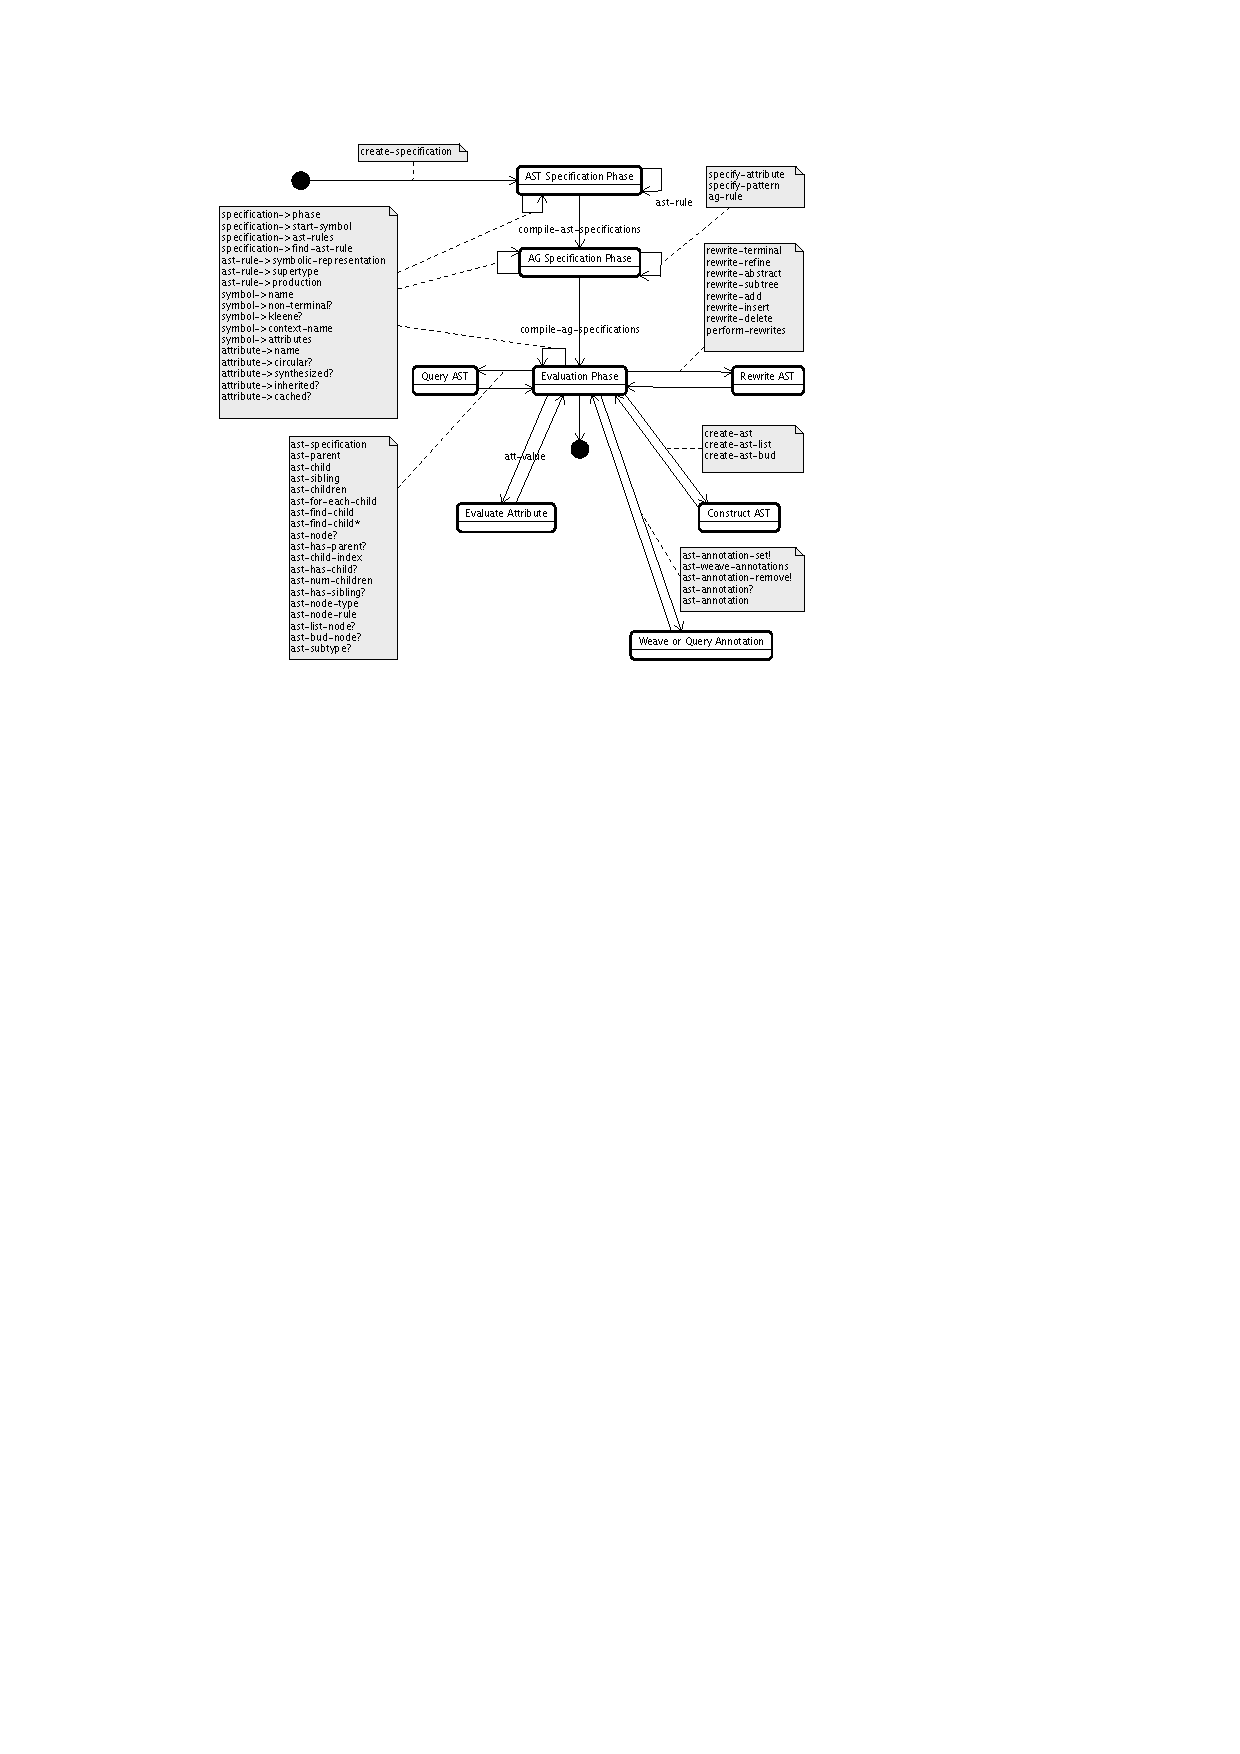
\includegraphics[width=0.9\linewidth]{../../documentation/figures/user-interface.pdf}
	\caption[Die RACR API]{RACR API~\cite{Buerger2012}}
	\label{fig:racr-api}
\end{figure}

%RACR macht sich zwei prägende Programmier-Paradigmen von Scheme zu eigen: RACR ist prozedural. Es existiert kein fester Zusammenhalt zwischen Daten und Funktionen, wie es bei der objektorientierten Programmierung der Fall ist. In der Scheme-Implementierung von RACR werden zur Speicherung der Spezifikationen und AST-Knoten bestimmte Scheme"=Records angelegt. RACR-spezifische Typen sind opak: Auf die einzelnen Felder dieser Records kann von außerhalb der RACR-Bibliothek nicht direkt zugegriffen werden. Ihr Aufbau widerspiegelt sich nicht in der Schnittstelle. Die wichtigsten RACR-spezifischen Datentypen sind \scm{racr-specification} und \scm{node}. RACR bietet Prozeduren, die diese Datenstrukturen zu erzeugen, und die auf sie angewandt werden können. Des Weiteren is RACR funktional. Einige Prozeduren RACRs erwarten eine Prozedur als Parameter. Dies betrifft vor allem die Attributsspezifikation.

\section{Das .NET-Framework und die Common Language Infrastructure}\label{sec:cli}

.NET ist ein von Microsoft entwickeltes Software-Framework und eine integrale Komponente des Windows-Betriebssystems. Für .NET entwickelte Programme werden nicht direkt nach Machinencode, sondern nach Bytecode – der Intermediate Language (IL) – übersetzt und laufen innerhalb eines virtuellen Ausführungssystems. Programmiersprachen, die nach IL kompilieren, werden .NET-Sprachen genannt, wobei C\# und Visual Basic .NET zu den wichtigsten Vertretern gehören. Der IL-Code wird in sogenannten Assemblies in Form von EXE-Dateien (Prozess-Assemblies) oder DLL-Dateien (Library-Assemblies) gespeichert.

Die stapelbasierende virtuelle Maschine (VM) von .NET wird innerhalb der Common Language Infrastructure (CLI)~\cite{ECMA2012}, einem internationalen Standard, definiert und bietet sprach-neutrale Features, wie zum Beispiel automatische Speicherbereinigung, Exceptions, Typsicherheit, Zugriff auf eine umfangreiche Klassenbibliothek und Just-in-Time-Kompilierung, wobei entsprechend der zu Grunde liegenden Rechnerarchitektur IL-Code bedarfsgesteuert zu nativem Code übersetzt wird. Neben der Common Language Runtime (CLR), der Microsoft-Implementierung der CLI, existieren Portable.NET\footnote{\url{http://www.dotgnu.org/}} und das Mono-Projekt\footnote{\url{http://www.mono-project.com/}} als kompatible, quelloffene Alternativen.

\begin{figure}
	\centering
	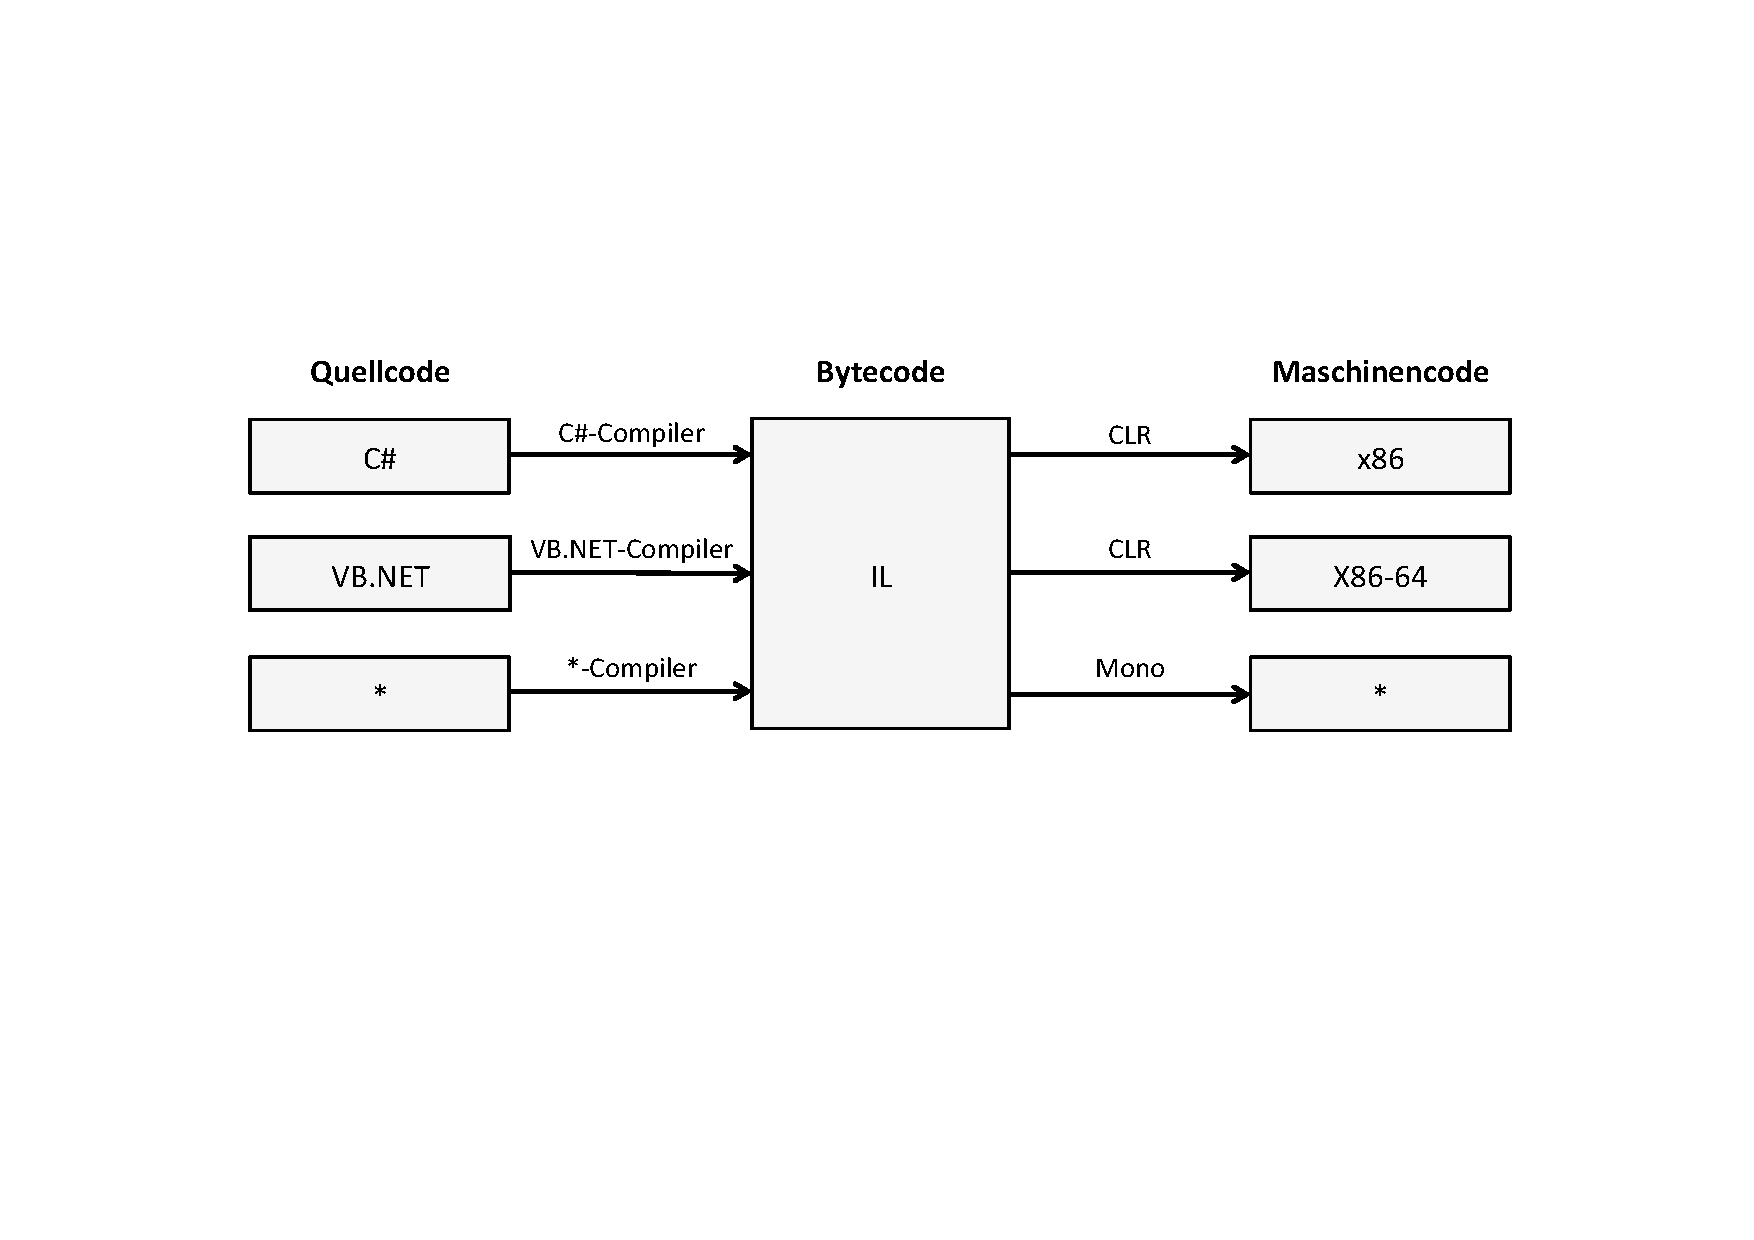
\includegraphics[width=0.9\linewidth]{figures/common-language-infrastructure.pdf}
	\caption{Übersetzung von .NET-Sprachen nach Maschinencode}
	\label{fig:cli}
\end{figure}

Abbildung~\ref{fig:cli} veranschaulicht die Kompillierungsprozesse, die der Ausführung eines .NET-Programms vorhergehen müssen. Alle .NET-Programme haben gleichen Bytecode, unabhängig von der Implementierungssprache oder der Zielarchitektur. Dies hat folgende wichtige Konsequenzen zur Folge:

\begin{itemize}
	\item .NET-Programme sind nicht architekturgebunden, sondern plattformunabhängig. Ein unter Windows entwickeltes Programm kann nach der Kompilierung unter Linux (mittels Mono) ausgeführt werden und umgekehrt.
	\item .NET-Sprachen haben zueinander hohe Interoperabilität. Die CLI vereinheitlicht unter anderem Exception-Handling, den Aufbau von und Zugriff auf Klassenbibliotheken und die Interaktion zwischen allen Datentypen. Objektinstanzen können über Sprachgrenzen hinweg ausgetauscht werden.
\end{itemize}

\section{IronScheme}

IronScheme\footnote{\url{http://ironscheme.codeplex.com/}} ist eine quelloffene, weitgehend R6RS-konforme Scheme-Implementierung für die .NET Software-Plattform. Sie umfasst einen eigenständigen, interaktiven Interpreter zur Ausführung von Scheme-Programmen und eine Klassenbibliothek, mittels welcher IronScheme in andere .NET-Projekte eingebunden werden kann. Diese Klassenbibliothek erlaubt es, .NET–Strings\footnote{Genauer gesagt handelt es sich um den Typ \csh{System.String} – die Klasse \csh{String} im Namensraum \csh{System}.} als Scheme-Ausdruck auszuwerten, analog zu der \scm{Eval}-Funktion, wie sie in vielen dynamischen Sprachen zu finden ist. So wird während der Programmausführung aus dem Scheme-Code IL-Code generiert und dieser anschließend ausgeführt. Scheme-Bibliotheken können jedoch auch zu Assemblies vorkompiliert werden.

\begin{table}[h!]
	\centering
	\begin{tabular}{@{}ll@{}}
		\toprule
			Scheme & .NET \\
		\midrule
			{\scm|fixnum|}		& {\csh|System.Int32|}			\\
			{\scm|flonum|}		& {\csh|System.Double|}			\\
			{\scm|boolean|}		& {\csh|System.Boolean|}		\\
			{\scm|string|}		& {\csh|System.String|}			\\
			{\scm|pair|}		& {\csh|IronScheme.Runtime.Cons|}	\\
			{\scm|'()|}		& {\csh|null|}				\\
			{\scm|hashtable|}	& {\csh|System.Collections.Hashtable|}	\\
			{\scm|symbol|}		& {\csh|Microsoft.Scripting.SymbolId|}	\\
			{\scm|procedure|}	& {\csh|Ironscheme.Runtime.Callable|}	\\
		\bottomrule		
	\end{tabular}
	\caption{IronSchemes Abbildung von Scheme-Datentypen auf .NET-Datentypen}
	\label{tab:typemapping}
\end{table}

Viele wichtige Datentypen sind als Adapter für .NET-Datentypen realisiert, was die Interoperabilität von IronScheme zu anderen .NET"=Sprachen erhöht. Andere Datentypen implementieren spezielle Schnittstellen. Die für diese Arbeit relevanten Scheme-Typen und deren zugehörige .NET-Typen sind in Tabelle~\ref{tab:typemapping} aufgeführt.
